
\chapter{Level1B data format and quality}


\section{Data format}

\smr\ Level0 and Level1B data are stored in tables
in a calibration database at the Dept. of Earth and Space
Sciences at Chalmers University of Technology (Chalmers) in Gothenburg.
There are several ways to access the data but the recommendation is to access
data through the \smr\ web-page \url{http://malachite.rss.chalmers.se}. 
On the \smr\ web-page Level1b and auxiliary data are basically displayed in three different
views (frequency mode view, scan info view, and scan data view), as explained below:
\begin{enumerate}

\item Frequency mode view: displays which frequency modes that were deployed for a
 given date in Json format. Example URL
 \url{http://malachite.rss.chalmers.se/rest_api/v3/freqmode_info/2015-01-03/} and content
 \begin{tiny}
 \begin{verbatim}
 {
  "Date": "2015-01-03", 
  "Info": [
    {
      "Backend": "AC1", 
      "FreqMode": 2, 
      "NumScan": 481, 
      "URL": "http://malachite.rss.chalmers.se/rest_api/v3/freqmode_info/2015-01-03/AC1/2"
    }, 
    {
      "Backend": "AC1", 
      "FreqMode": 21, 
      "NumScan": 241, 
      "URL": "http://malachite.rss.chalmers.se/rest_api/v3/freqmode_info/2015-01-03/AC1/21"
    }, 
    {
      "Backend": "AC2", 
      "FreqMode": 1, 
      "NumScan": 481, 
      "URL": "http://malachite.rss.chalmers.se/rest_api/v3/freqmode_info/2015-01-03/AC2/1"
    }, 
    {
      "Backend": "AC2", 
      "FreqMode": 8, 
      "NumScan": 125, 
      "URL": "http://malachite.rss.chalmers.se/rest_api/v3/freqmode_info/2015-01-03/AC2/8"
    }, 
    {
      "Backend": "AC2", 
      "FreqMode": 17, 
      "NumScan": 122, 
      "URL": "http://malachite.rss.chalmers.se/rest_api/v3/freqmode_info/2015-01-03/AC2/17"
    }
  ]
}
 \end{verbatim}
\end{tiny}
For this date it can be seen that five different frequency modes (FreqMode) were deployed.
For each frequency mode an URL is given where more detailed information of
the scans (NumScan=number of scans) from this date can be obtained, as explained below.
 

\item scan info view: displays log data in Json format for each scan from a given date and frequency mode. 
  As example, the URL \url{http://malachite.rss.chalmers.se/rest_api/v3/freqmode_info/2015-01-03/AC1/2/}
  displays scan info data for all frequency mode 2 measurements from 2015-01-03 
  and the data for the first scan is shown below (the fields are 
   described in Table~\ref{table:logdataformat}):
\begin{tiny}
 \begin{verbatim}
 {
  "Info": [
    {
      "AltEnd": 4905.25, 
      "AltStart": 94420.199999999997, 
      "DateTime": "Sat, 03 Jan 2015 09:48:23 GMT", 
      "EndLat": -74.942700000000002, 
      "EndLon": 128.27600000000001, 
      "FirstSpectrum": 7002890483, 
      "FreqMode": 2, 
      "LastSpectrum": 7002892467, 
      "MJD": 57025.408605249999, 
      "NumSpec": 32, 
      "ScanID": 7002887494, 
      "StartLat": -84.495999999999995, 
      "StartLon": 134.69, 
      "SunZD": 68.722450000000009, 
      "URL": "http://malachite.rss.chalmers.se/rest_api/v3/scan/AC1/2/7002887494", 
      "URL-apriori-BrO": "http://malachite.rss.chalmers.se/rest_api/v3/apriori/BrO/2015-01-03/AC1/2/7002887494", 
      "URL-apriori-C2H2": "http://malachite.rss.chalmers.se/rest_api/v3/apriori/C2H2/2015-01-03/AC1/2/7002887494", 
      "URL-apriori-C2H6": "http://malachite.rss.chalmers.se/rest_api/v3/apriori/C2H6/2015-01-03/AC1/2/7002887494", 
      "URL-apriori-CH3CN": "http://malachite.rss.chalmers.se/rest_api/v3/apriori/CH3CN/2015-01-03/AC1/2/7002887494", 
      "URL-apriori-CH3Cl": "http://malachite.rss.chalmers.se/rest_api/v3/apriori/CH3Cl/2015-01-03/AC1/2/7002887494", 
      "URL-apriori-CH4": "http://malachite.rss.chalmers.se/rest_api/v3/apriori/CH4/2015-01-03/AC1/2/7002887494", 
      "URL-apriori-CO": "http://malachite.rss.chalmers.se/rest_api/v3/apriori/CO/2015-01-03/AC1/2/7002887494", 
      "URL-apriori-CO2": "http://malachite.rss.chalmers.se/rest_api/v3/apriori/CO2/2015-01-03/AC1/2/7002887494", 
      "URL-apriori-COF2": "http://malachite.rss.chalmers.se/rest_api/v3/apriori/COF2/2015-01-03/AC1/2/7002887494", 
      "URL-apriori-Cl2O2": "http://malachite.rss.chalmers.se/rest_api/v3/apriori/Cl2O2/2015-01-03/AC1/2/7002887494", 
      "URL-apriori-ClO": "http://malachite.rss.chalmers.se/rest_api/v3/apriori/ClO/2015-01-03/AC1/2/7002887494", 
      "URL-apriori-ClONO2": "http://malachite.rss.chalmers.se/rest_api/v3/apriori/ClONO2/2015-01-03/AC1/2/7002887494", 
      "URL-apriori-ClOOCl": "http://malachite.rss.chalmers.se/rest_api/v3/apriori/ClOOCl/2015-01-03/AC1/2/7002887494", 
      "URL-apriori-H2CO": "http://malachite.rss.chalmers.se/rest_api/v3/apriori/H2CO/2015-01-03/AC1/2/7002887494", 
      "URL-apriori-H2O": "http://malachite.rss.chalmers.se/rest_api/v3/apriori/H2O/2015-01-03/AC1/2/7002887494", 
      "URL-apriori-H2O2": "http://malachite.rss.chalmers.se/rest_api/v3/apriori/H2O2/2015-01-03/AC1/2/7002887494", 
      "URL-apriori-H2S": "http://malachite.rss.chalmers.se/rest_api/v3/apriori/H2S/2015-01-03/AC1/2/7002887494", 
      "URL-apriori-HBr": "http://malachite.rss.chalmers.se/rest_api/v3/apriori/HBr/2015-01-03/AC1/2/7002887494", 
      "URL-apriori-HCN": "http://malachite.rss.chalmers.se/rest_api/v3/apriori/HCN/2015-01-03/AC1/2/7002887494", 
      "URL-apriori-HCOOH": "http://malachite.rss.chalmers.se/rest_api/v3/apriori/HCOOH/2015-01-03/AC1/2/7002887494", 
      "URL-apriori-HCl": "http://malachite.rss.chalmers.se/rest_api/v3/apriori/HCl/2015-01-03/AC1/2/7002887494", 
      "URL-apriori-HF": "http://malachite.rss.chalmers.se/rest_api/v3/apriori/HF/2015-01-03/AC1/2/7002887494", 
      "URL-apriori-HI": "http://malachite.rss.chalmers.se/rest_api/v3/apriori/HI/2015-01-03/AC1/2/7002887494", 
      "URL-apriori-HNO3": "http://malachite.rss.chalmers.se/rest_api/v3/apriori/HNO3/2015-01-03/AC1/2/7002887494", 
      "URL-apriori-HO2": "http://malachite.rss.chalmers.se/rest_api/v3/apriori/HO2/2015-01-03/AC1/2/7002887494", 
      "URL-apriori-HOBr": "http://malachite.rss.chalmers.se/rest_api/v3/apriori/HOBr/2015-01-03/AC1/2/7002887494", 
      "URL-apriori-HOCl": "http://malachite.rss.chalmers.se/rest_api/v3/apriori/HOCl/2015-01-03/AC1/2/7002887494", 
      "URL-apriori-N2": "http://malachite.rss.chalmers.se/rest_api/v3/apriori/N2/2015-01-03/AC1/2/7002887494", 
      "URL-apriori-N2O": "http://malachite.rss.chalmers.se/rest_api/v3/apriori/N2O/2015-01-03/AC1/2/7002887494", 
      "URL-apriori-NH3": "http://malachite.rss.chalmers.se/rest_api/v3/apriori/NH3/2015-01-03/AC1/2/7002887494", 
      "URL-apriori-NO": "http://malachite.rss.chalmers.se/rest_api/v3/apriori/NO/2015-01-03/AC1/2/7002887494", 
      "URL-apriori-NO2": "http://malachite.rss.chalmers.se/rest_api/v3/apriori/NO2/2015-01-03/AC1/2/7002887494", 
      "URL-apriori-O2": "http://malachite.rss.chalmers.se/rest_api/v3/apriori/O2/2015-01-03/AC1/2/7002887494", 
      "URL-apriori-O3": "http://malachite.rss.chalmers.se/rest_api/v3/apriori/O3/2015-01-03/AC1/2/7002887494", 
      "URL-apriori-OBrO": "http://malachite.rss.chalmers.se/rest_api/v3/apriori/OBrO/2015-01-03/AC1/2/7002887494", 
      "URL-apriori-OCS": "http://malachite.rss.chalmers.se/rest_api/v3/apriori/OCS/2015-01-03/AC1/2/7002887494", 
      "URL-apriori-OClO": "http://malachite.rss.chalmers.se/rest_api/v3/apriori/OClO/2015-01-03/AC1/2/7002887494", 
      "URL-apriori-OH": "http://malachite.rss.chalmers.se/rest_api/v3/apriori/OH/2015-01-03/AC1/2/7002887494", 
      "URL-apriori-SF6": "http://malachite.rss.chalmers.se/rest_api/v3/apriori/SF6/2015-01-03/AC1/2/7002887494", 
      "URL-apriori-SO2": "http://malachite.rss.chalmers.se/rest_api/v3/apriori/SO2/2015-01-03/AC1/2/7002887494", 
      "URL-ptz": "http://malachite.rss.chalmers.se/rest_api/v3/ptz/2015-01-03/AC1/2/7002887494"
    },
 .
 . # in this example only data from one scan is displayed
 . 
 }  
\end{verbatim}
\end{tiny}
As can be seen, the data structure contains a number of URLs. These URLs displays more detailed
data (Level1B and auxiliary data) as described below.


\item scan data view: displays Level1B and auxiliary data in Json format for a scan.
Three different views are available, and example URLS are give below: 
\begin{itemize}
\item for Level1B \url{http://malachite.rss.chalmers.se/rest_api/v3/scan/AC1/2/7002887494/},
     Table~\ref{table:dataformat} gives a description of the data fields.

\item for PTZ data (pressure,temperature, and altitude data) 
\url{malachite.rss.chalmers.se/rest_api/v3/ptz/2015-01-03/AC1/2/7002887494}
 Table~\ref{table:ptzdataformat} gives a description of the data fields.

\item for \textit{a priori} \chem{O_{3}} data 
\url{http://malachite.rss.chalmers.se/rest_api/v3/apriori/O3/2015-01-03/AC1/2/7002887494/},
(see the scan info view above for other available \textit{a priori} data).
 Table~\ref{table:aprioridataformat} gives a description of the data fields.
 
\end{itemize}
	

\end{enumerate}

\begin{longtable}{| p{.20\textwidth} | p{.70\textwidth} |}
\hline
  \textbf{Variable} & \textbf{Description} \\
  \hline
    AltEnd                & tangent point altitude ([\,m\,]) for last spectrum in scan \\ \hline
    AltStart              & tangent point altitude for first spectrum in scan \\ \hline
    DateTime              & mean datetime (datetime(firts) + datatime(last))/2 of scan \\ \hline
    EndLat                & latitude of tangent point for last spectrum in scan \\ \hline
    EndLon                & longitude of tangent point for last spectrum in scan \\ \hline
    FirstSpectrum         & satellite time word for first spectrum in scan \\ \hline
    FreqMode              & deployed frequency mode \\ \hline
    LastSpectrum          & satellite time word for last spectrum in scan \\ \hline
    MJD                   & mean modified julian date (MJD(first) + MJD(last))/2 of scan \\ \hline
    NumSpec               & number of atmospheric spectra in scan \\ \hline
    ScanID                & satellite time word identifier of scan\\ \hline
    StartLat              & latitude at tangent point for first spectrum in scan \\ \hline
    StartLon              & longitude at tangent point for first spectrum in scan \\ \hline
    SunZD                 & mean solar zenith angle  (SunZD(first) + SunZD(last))/2 for scan\\ \hline
\hline
\caption{ Odin scan log data data format. Latitudes and longitudes are given as geodetic
coordinates using WGS84 reference ellipsoid.}
\label{table:logdataformat}
\end{longtable}


  

%A description of how to access the data
%is given on the Odin web-page. Table~\ref{table:dataformat} gives a description 
%of the \smr\ Level1B v8 scan data format.
 \lcomment{BR}{fill in descriptions and remove unnecessary data}

\begin{longtable}{| p{.20\textwidth} | p{.70\textwidth} |} 
\hline
  \textbf{Variable} & \textbf{Description} \\
  \hline
     Version         & calibration version \\ \hline
     Level           & \\ \hline
     Quality         & Quality indicator of scan/spectrum (see Table~\ref{table:quality}) \\ \hline
     STW             & satellite time word\\ \hline
     MJD             & Modified julian date of observation \\ \hline
     Orbit           & Number of orbit plus fraction \\ \hline
     LST             & Local sidereal time [s] of observation \\ \hline
     Source          & \\ \hline
     Discipline      & \\ \hline
     Topic           & \\ \hline
     Spectrum        & Frequency sorted spectra, which can be of three types\\
                     & - Receiver noise temperature spectrum\\
                     & - SSB spectrum\\
                     & - Intenisty calibrated spectrum in Rayleigh Jeans temperature in Kelvin\\    
                     & (N.B. use "Type" to distinguish between type of spectrum) )\\ \hline
     ObsMode         & \\ \hline
     Type            & Type of spectrum (3=Trec, 8=atmospheric,9=SSB)\\ \hline
     Frontend        & The frontend used for this observation: 1=555, 2=495, 3=572, 4=549, 5=119\\ \hline
     Backend         & The backend used for this observation: 1=AC1, 2=AC2\\ \hline
     SkyBeamHit      & The 16 bits of this word indicate possible hits of major
                       sources of submillimetre emission by one of the skybeams or the
                       main beam. E.g to test if the main beam was pointing at the Moon
                       when a spectrum was taken during a limb scan measurement in aeronomy
                       mode:
                       MOONMB:  0x0200\\ \hline
     RA2000          & The right ascension (J2000) of the direction of pointing in degrees. \\ \hline
     Dec2000         & The declination (J2000) of the direction of pointing in degrees. \\ \hline
     VSource         & \\ \hline
     Longitude       & Geodetic latitude of the tangent point.\\ \hline
     Latitude        & Geodetic latitude of the tangent point.\\ \hline
     Altitude        & Tangent point altitude [m].\\ \hline
     Qtarget         & The reference attitude given as a quaternion (4-vector).\\ \hline
     Qachieved       & The achieved attitude given as a quaternion (4-vector).\\ \hline
     Qerror          & The attitude error in degrees, describing the pointing uncertainty
                       around the 3 principle axes of the satellite. \\ \hline
     GPSpos          & The geocentric position $X$,$Y$,$Z$ in meter of the satellite.\\ \hline
     GPSvel          & The geocentric velocity $\dot X$, $\dot Y$, $\dot Z$ in meter per 
                         second of the satellite.\\ \hline
     SunPos          & The geocentric position of the Sun in meter.\\ \hline
     MoonPos         & The geocentric position of the Moon in meter.\\ \hline
     SunZD           & The solar zenith angle in degrees. \\ \hline
     Vgeo            & The velocity of the satellite with respect to the Earth in meter per second.\\ \hline
     Vlsr            & \\ \hline
     Tcal            & The temperature in Kelvin of the calibration load.\\ \hline
     Tsys            & The mean value of the receiver nosie temperature in Kelvin used during the intensity calibration.\\ \hline
     SBpath          & The path length in meter of the SSB diplexer. \\ \hline
     LOFreq          & Local oscillator frequency in Hz in the rest frame of the satellite.\\ \hline
     SkyFreq         & The frequency in Hz of the centre channel in the rest frame of the
                         satellite, i.e not Doppler corrected.\\ \hline
     RestFreq        & The frequency in Hz of the centre channel in the rest frame of the
                         observed object, i.e Doppler corrected.\\ \hline
     MaxSuppression  & The sideband frequency in Hz corresponding to the frequency of
                        maximum suppression in the rest frame of the satellite,
                        i.e not Doppler corrected.\\ \hline
     AttitudeVersion & The version number of the attitude reconstruction software (SODA) 
                         used at SSC during production of attitiude files.\\  \hline
     FreqRes         & The spacing in Hz between neighbouring channels for this spectrum. \\ \hline
     FreqCal         & these are the four local oscillator frequencies of the SSB modules\\ \hline
     IntMode         & \\ \hline
     IntTime         & The integration time in seconds, i.e. the duration of this observation.\\ \hline
     EffTime         & The effective integration time in seconds, i.e. you will get the
                         noise level in this spectrum by using this time and the receiver noise 
                         temperature from above and the usual radiometer formula:
                        \begin{verbatim}dT = Tsys/sqrt(df * EffTime)\end{verbatim}
                         where {\tt df} is the bandwidth of the spectrometer.\\ \hline
     Channels        & The number of channels in this spectrum.\\ \hline
     FreqMode        & Frequency mode applied\\ \hline
     TSpill          & Estimated Tspill in Kelvin \\ \hline
     ScanID          & satellite time word scan identifier\\ \hline
     Frequency       & This information can be used to create a frequency grid for the spectrum.
                       This field consists of three fields: IFreqGrid, LOFreq, and SSB.
                       The frequency grid can be obtained by
                       \begin{verbatim}frequency = LOFreq + IFreqGrid\end{verbatim}
                       The SSB data can be used to identify from which sub-band a given
                       channel belongs to, in s frequency sorted spectrum. 
                       An example SSB data is [1, -1, -1, 2, -1, -1, 3, 420, 508, 4, 509, 618, 5, 111, 199, 6, 1, 110, 7, 310, 419, 8, 200, 309].
                       Every third index (starting from first) corresponds to a band number.
                       The two following indexes describes the min and max indexes of the frequency sorted spectrum that
                       belongs to that band. -1 -1 indicates that data from this band is not used.  \\ \hline
     ZeroLagVar      & Zerolag variation of the surrounding reference measurements for all sub-bands.
                       \begin{verbatim}ZeroLagVar = abs(diff(ZeroLag))/mean(ZeroLag)\end{verbatim}
                        ZeroLag is the measured coefficient of the first channel of the auto-correlator,
                        and is proportional to the total power of the band. \\ \hline
\hline
\caption{ \smr\ scan data format.}
\label{table:dataformat}
\end{longtable}

\begin{longtable}{| p{.20\textwidth} | p{.70\textwidth} |}
\hline
  \textbf{Variable} & \textbf{Description} \\
  \hline
    P               & pressure vector ([\,hPa\,])  \\ \hline
    T               & temperature vector([\,K\,]) \\ \hline
    Z               & altitude vector([\,m\,]) \\ \hline
    datetime        & mean datetime of scan \\ \hline
    latitude        & mean latitude of scan \\ \hline
    longitude       & mean longitude of scan\\ \hline
    ScanID          & satellite time word identifier of scan \\ \hline
\hline
\caption{ \smr\ PTZ data data format.}
\label{table:ptzdataformat}
\end{longtable}


\begin{longtable}{| p{.20\textwidth} | p{.70\textwidth} |}
\hline
  \textbf{Variable} & \textbf{Description} \\ \hline
    day\underline{ }of\underline{ }year     & day of year  \\ \hline
    latitude        & mean latitude of scan  \\ \hline
    pressure        & pressure vector([\,Pa\,]) \\ \hline
    source          & filename \\ \hline
    species         & species, text, e.g. \chem{O_{3}}  \\ \hline
    vmr             & volume mixing ratio vector\\ \hline
\hline
\caption{ \smr\ \textit{a priori} data data format.}
\label{table:ptzdataformat}
\end{longtable}



\section{Quality flags}

The Quality variable of an \smr\ Level1B structure is a scalar value.
The value is determined from a quality control
of both scan variables and the individual spectrum.
Each test performed (see Table~\ref{table:quality}) is related to a unique scalar value
and the Quality variable is the sum of the values of tests 
that were not passed.  
Thus, a spectrum with a Quality value of 0 is best.

The radiometric noise of the spectra of a scan is estimated as decribed  
in Sect.~\ref{sec:radper} (and reported as an effective integration time (EffTime)).
This estimate does not contain the broadband noise (due to gain variation). 
The scan data contains the variable ZeroLagVar which can be seen as an estimate
of the broadband gain variation (ZeroLagVar\(\approx \frac{\Delta g}{g}\) [\%]) 
of the two surrounding references of a target spectrum. 
\lcomment{BR}{add description of how this variable can be used to estimate broadband 
noise level uncertainty}
 

\begin{longtable}{| p{.30\textwidth} | p{.50\textwidth} | p{.10\textwidth} |}
  \hline
  \textbf{Test} & \textbf{Description} & \textbf{Value} \\
  \hline
  check of Tspill   & outside of valid range (3--12\,K) & 0x0001 \\
  \hline
  check of Trec     & outside of valid range (2000--4000\,K) & 0x0002  \\
  \hline
  check of Noise    & outside of valid range (0.5-6\,K) & 0x0004  \\
  \hline
  check of Scanning & tangent altitude is not decreasing or increasing as expected & 0x0008 \\
  \hline
  check of nr of Spectra &  the scan consists of less than five spectra & 0x0010\\
  \hline
  check of Tb       & outside of valid range (-15 -- 280\,K) & 0x0020\\ 
  \hline
  check of Tint     & integration time is outside valid range (0.5--10\,s) & 0x0040\\
  \hline
  check of References 1 & atmospheric spectrum is not collected between two sky beam 1 references     & 0x0080\\
  \hline
  check of References 2 & surrounding references have different & 0x0100\\
                        & integration times                     & \\ 
  \hline check of Moon hit   & the moon is in the main beam          & 0x0200 \\

\hline
\caption{ Description of the \smr\ Quality variable. }
\label{table:quality}
\end{longtable}



%\begin{figure}[t]
%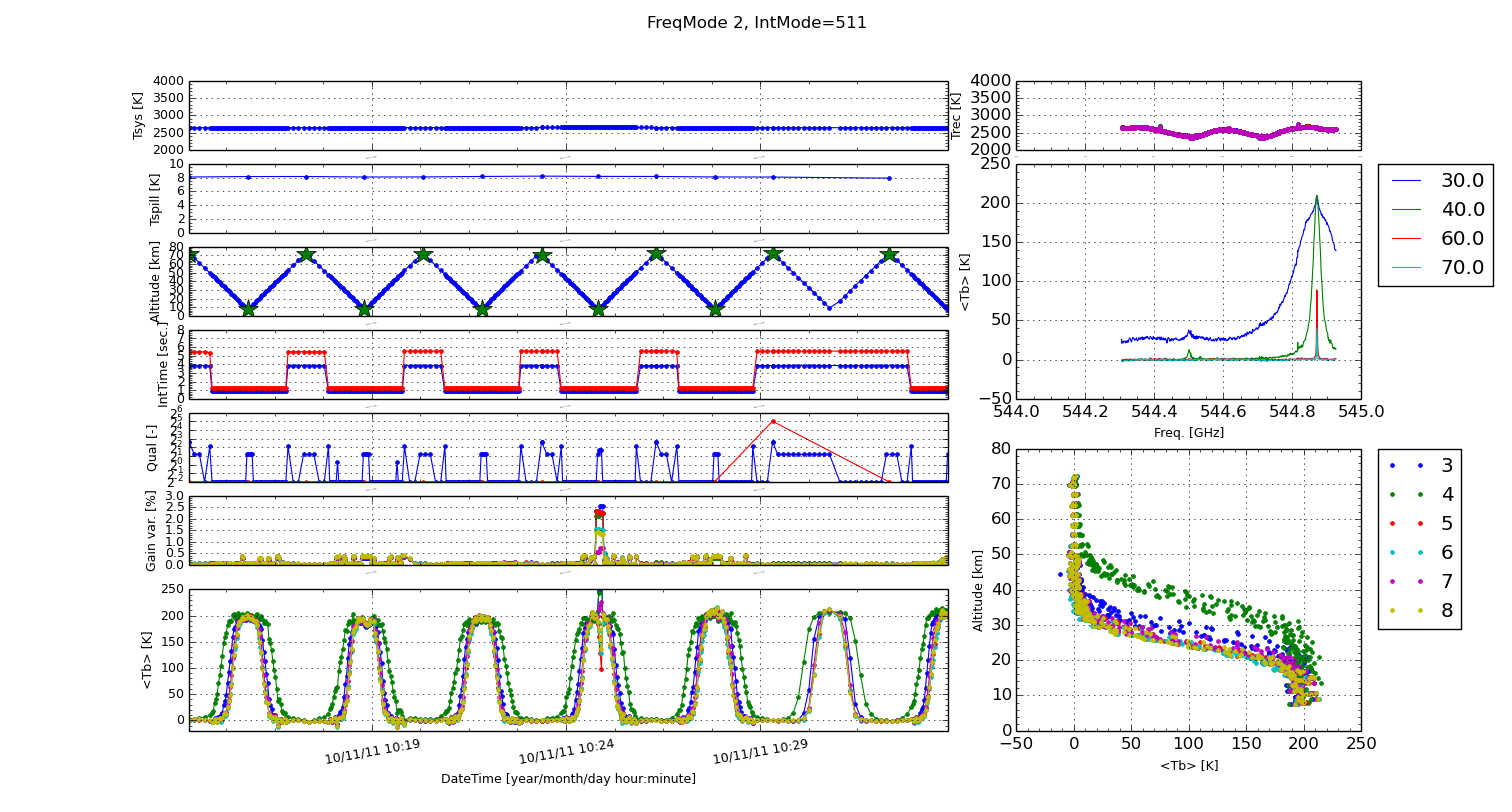
\includegraphics[width=14cm]{quality_control.png}
%\caption{Quality flag example figure\lcomment{BR}{update or remove }}
%\label{fig:quality}
%\end{figure}

    




\chapter{Summary}


Some key issues that should be considered when examining or applying \smr\
Level1B data:
\begin{itemize}

\item \smr\ can perform observations in a number of different frequency
bands, mainly within the 486\,--\,504\,GHz and 541\,--\,581\,GHz regions.
In practise, two or three frequency bands are measured simultaneously.
For a given day, several observation modes can be applied, and hence
it is rather complicated to describe the time-sharing in a 
comprehensive way.
 

\item Calibrated spectra are expressed in terms of Rayleigh--Jeans brightness temperature.

\item \smr\ spectra contain a significant amount of broadband noise, 
due to rapid gain fluctuations, in addition to radiometric noise.


\end{itemize}

